\documentclass[a4paper,11pt]{article}
\usepackage{a4wide}
\usepackage{geometry}
  \geometry{paper=a4paper,top=2.2cm,bottom=2.9cm}
   \geometry{right=2.3cm,left=2.3cm}
% Feynman diagrammen
\usepackage{feynmp}
\unitlength = 1mm
% Afbeeldingen
\usepackage{graphicx} % afbeeldingen
\usepackage{subfigure} % pakket voor het gebruiken van sub-figuren
\usepackage{float} % laat toe [H] te gebruiken bij plaatsen figuren
% Taal
\usepackage[dutch]{babel}
%\hyphenation{}
% De formules
\usepackage{amssymb, amsmath} % wiskunde
\numberwithin{equation}{section} % (#.#) i.p.v. (#)
% xetex
\usepackage{fontspec}
\usepackage{xunicode}
\usepackage{xltxtra}
\setromanfont[Mapping=tex-text]{Calibri}
% appendix
\usepackage{appendix}


\title{Dwarse energiestroom in de LHeC met saturatie}
\author{Ruben Van Boxem}

\begin{document}

% titelpagina
\fontsize{12pt}{14pt}\selectfont

\begin{center}


\includegraphics[height=3cm]{Afbeeldingen/UA.eps}

\vspace{1cm}

\fontsize{14pt}{17pt}\selectfont
% De Faculteit:
\textsc{Faculteit Wetenschappen} \\
\textsc{Departement Fysica}
\fontsize{12pt}{14pt}\selectfont
\vspace{0.3cm}

\vspace{1.2cm}

%Het academiejaar: aanpassen!
Academiejaar 2009--2010

\vspace{2.8cm}

\fontsize{17.28pt}{21pt}\selectfont

% De titel van de thesis:
\textsc{Dwarse energiestroom in de LHeC met saturatie}

\fontseries{m}
\fontsize{12pt}{14pt}\selectfont

\vspace{3cm}

% De auteur van de thesis:
Ruben \textsc{Van Boxem}	


\vspace{2cm}

Promotor: Prof. Dr Pierre \textsc{Van Mechelen}\\
Copromotor: Krzysztof \textsc{Kutak} \\
\vspace{2cm}
\end{center}
% De functie van de thesis:
Proefschrift voorgedragen tot \\
het behalen van de graad van\\
\textsc{Bachelor in de Fysica}


\thispagestyle{empty}
\newpage

\section*{Dankwoord}
TODO
\thispagestyle{empty}
\newpage
\fontsize{11pt}{14pt}\selectfont

\section*{Summary}
TODO
\thispagestyle{empty}
\newpage

\tableofcontents
\thispagestyle{empty}
\newpage

\section{Diepe inelastische verstrooiing}
      \paragraph{}
Om de diepere structuur van een object zoals het proton te bestuderen, kan men elektron verstrooiing gebruiken.
Door middel van een elektron met hoge energie op een proton te laten botsen kan men de onderliggende samenstelling van het proton bestuderen.
Een proces dat zich hier goed voor leent, heet DIS, oftewel \textit{Deep Inelastic Scattering}. In figuur \ref{fig:DIS} wordt een DIS proces schematisch weergegeven.
\begin{figure} [H]
  \begin{center}
    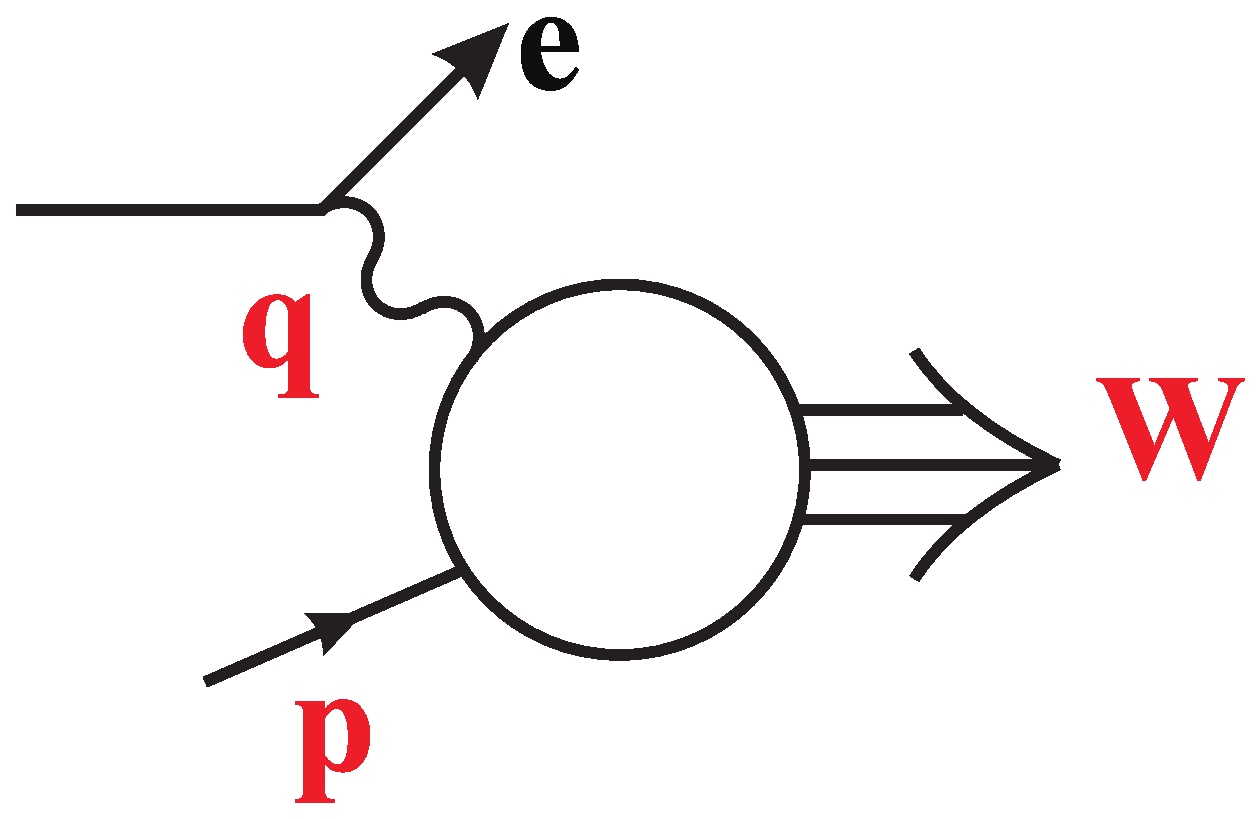
\includegraphics[width=.33\textwidth]{Afbeeldingen/DIS.eps}
    \caption{Elektron-proton verstrooiing.
Het elektron zendt een boson uit dat het proton “onderzoekt".
$P$ is de vierimpuls van het inkomend proton, $W$ is de invariante massa van het uitgaande systeem (dus zonder elektron), $q$ is de overgedragen vierimpuls. \cite{Martin}}
   \label{fig:DIS}
  \end{center}
\end{figure}
 Men spreekt van DIS processen als $Q^2 \gg M^2$ (“diep”) en $W^2 = (P+q)^2 \gg M^2$ (“inelastisch”).
Omdat de waarde van $q^2$ negatief is, wordt vaak volgende variabele ingevoerd: $Q^2 :=-q^2 > 0$. De golflengte van het het foton is van de grootteorde van $1/Q$.
Dit wil concreet zeggen dat als de overgedragen impuls verhoogt, de golflengte van het foton en dus de grootte van de deeltjes waarmee het interageert, kleiner wordt.

      \paragraph{}
Men kan twee soorten DIS interacties onderscheiden: neutrale en geladen stroom (respectievelijk NC en CC). De Feynman diagrammen worden weergegeven in figuur \ref{fig:NC-CC}.
\begin{figure} [H]
  \centering
  \subfigure[NC interactie met uitwisseling van een foton of $Z$ boson.]{
  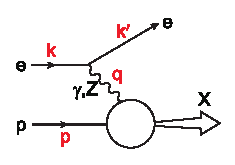
\includegraphics[width=.33\textwidth]{Afbeeldingen/NC.eps}
  \label{fig:NC}
  }
  \subfigure[CC interactie met uitwisseling van een $W^\pm$ boson.]{
  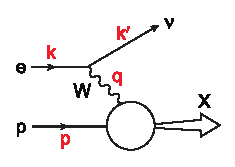
\includegraphics[width=.33\textwidth]{Afbeeldingen/CC.eps}
  \label{fig:CC}
  }
  \caption{Soorten DIS. \cite{Martin}}
  \label{fig:NC-CC}
\end{figure}

      \paragraph{}
In wat volgt wordt beschreven wat er gebeurt als men $Q^2$ systematisch verhoogt.

  \subsection{Breking van schaalinvariantie}
    \paragraph{Elektron-kern verstrooiing}
Stel dat een elektron verstrooid wordt op een atoomkern (bestaande uit meerdere nucleonen).
Als $\lambda \gg d_\text{kern}$, ziet het foton de kern als een puntdeeltje en wordt het elastisch verstrooid op een puntdeeltje met de lading van de kern.
Als $\lambda \ll d_\text{kern}$, dringt het foton diep door in de kern en kan het verstrooid worden op een proton in de kern.
Men spreekt hier van diep inelastische elektron-kern verstrooiing, en men kan het volgende schrijven:
\begin{align}
x_N = \frac{M}{M_N} \left( \frac{Q^2}{2M\nu} \right) = \frac{1}{A}
\end{align}
waarbij $M_N$ de massa van de kern is, $M$ de massa van het proton, $\nu$ de frequentie van het foton en $A$ het aantal nucleonen in de kern.
Als men de werkzame doorsnede van deze processen zou uitzetten t.o.v. $x_N$, ziet men een duidelijke verschil tussen de gevallen waar $\lambda \gg d_\text{kern}$ en die waar $\lambda \ll d_\text{kern}$.
Dit fenomeen heet \textit{schaalinvariantie}, waarbij de waargenomen werkzame doorsnede blijkbaar afhangt van de grootte van de schaal, $Q^2$.

      \paragraph{Elektron-proton verstrooiing}
Zolang dat $\lambda \gg d_\text{proton}$, ziet het foton het proton als puntdeeltje. Het wordt elastisch verstrooid door het proton.
Als $Q^2$ zo groot is dat $\lambda \ll d_\text{proton}$, wordt er opnieuw ``ingezoomd", waarbij het foton nu de bouwstenen van het proton kan “zien" (i.e. ermee kan interageren).
Het foton ziet dus de 3 quarks als puntdeeltjes en men spreekt van diep inelastische elektron-proton verstrooiing.
Kinematisch geldt het volgende (zie appendix \ref{app:DIS}):
\begin{align} \label{eq:Bjorkenx}
x = \left( \frac{Q^2}{2p\cdot q} \right)
\end{align}
$x$ wordt aangeduid als de “Bjorken schaalvariabele".
De waarschijnlijkheid van zo'n proces worden dus enkel en alleen bepaalt door $x$ en niet $Q^2$ en $p\cdot q$ afzonderlijk.

      \paragraph{Breking van schaalinvariantie}
In volgorde van stijgende $Q^2$ heeft men dus voor de werkzame doorsnede:
\begin{itemize}
  \item\textit{kern}schaling met een piek op $x_N=1$
  \item  breking van schaalinvariantie
  \item \textit{proton}schaling met een piek \textit{rond} $x \sim 1$
  \item breking van schaalinvariantie
  \item \textit{Bjorken}schaling met een \textit{uitgesmeerde} piek rond $x \sim 1/3$ (3 quarks)
\end{itemize}
Als men $Q^2$ blijft vergroten, verwacht men logischerwijs nogmaals een breking van schaalinvariantie te zien, en deze worden ook geobserveerd.
De schijnbare breking van schaalinvariantie ligt in lijn met de voorspellingen van QCD, de theorie van de sterke wisselwerking.

  \subsection{Zeequarks, gluonen en $\alpha_S$}
Quarks blijken niet uit een diepere structuur te bestaan (zodat er niet opnieuw een breking van schaalinvariantie optreedt).
In plaats van een diepere quark structuur, beschrijft QCD het proton als 3 valentiequarks (de klassieke $u u d$ combinatie) plus een willekeurig aantal zeequarks ($q\bar{q}$ paren).
Het foton ziet naast drie puntdeeltjes ook een zee van quarks.
Zeequarks ontstaan uit gluonen ($g\rightarrow q\bar{q}$) die zelf uitgestraald worden door andere quarks ($q\rightarrow gq$).
Het feit dat er extra deeltjes moeten bestaan in een proton volgt ook uit de experimentele waarneming dat slechts de helft van de impuls van het proton gedragen wordt door z’n valentiequarks.
Er treedt dus breking van schaalinvariantie op omdat elk parton (quark of gluon) bij een grotere waarde van $Q^2$, een kleiner deel  $x$ van de impuls $P$ van het proton zal dragen.
Deze breking van schaalinvariantie heeft volgende vorm:
\begin{align}
\alpha_S R \ln{\left( \frac{Q^2}{\mu^2}\right)}
\end{align}
Hier is $R$ een observabele en $\mu$ de renormalisatie schaal.
Merk op dat in tegenstelling tot de vorige brekingen van schaalinvariantie, deze logaritmisch is, wat bijzonder moeilijk te meten was toen deze ontdekking werd gedaan.

  \subsection{$\alpha_S$}
    \subsubsection{QED en $\alpha$} \label{sec:QED}
Om de vorm en het gedrag van de sterke koppeling te begrijpen, is het handig om eerst kort de koppeling in QED ($\alpha = e^2/4\pi$) te bekijken.
De processen die bijdragen aan een interactie van een foton met een enkel elektron worden in figuur \ref{fig:QED} weergegeven.
\begin{figure} [H]
  \begin{center}
    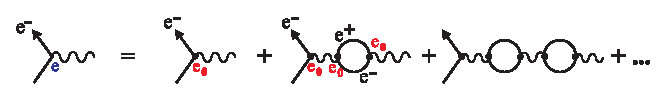
\includegraphics[width=.66\textwidth]{Afbeeldingen/QED.eps}
    \caption{Feynman diagrammen van de processen die bijdragen tot de interactie tussen een foton en een elektron. $e_0$ duidt hier op de naakte lading van het elektron.}
   \label{fig:QED}
  \end{center}
\end{figure}
De lading van een kaal elektron wordt afgeschermd door de “polarisatie van het vacuüm”, waardoor het foton extra $e^+ e^-$-paren “voelt”.
Hoe korter de golflengte van het foton, hoe meer $e^+ e^-$-paren het zal voelen.
Dit zorgt ervoor dat $\alpha$ toeneemt met $Q^2$.
De normalisatie van $\alpha$ komt uit vergelijking met experimentele data.
Algemeen kan men de elektromagnetische koppelingsfactor schrijven als volgt.
\begin{align}
\alpha(Q^2) = \alpha_0 \left[ 1+ \frac{\alpha_0}{3\pi} \ln{\frac{Q^2}{M^2}} + \left( \frac{\alpha_0}{3\pi} \ln{\frac{Q^2}{M^2}} \right)^2 +\hdots \right]
\end{align}
De \textit{loops} in de hogere orde Feynman diagrammen kunnen een oneindige bijdrage hebben indien er geen \textit{cut-off} waarde voor de \textit{loop}impuls wordt opgelegd.
Er wordt dus een renormalisatieschaal ingevoerd om de eindigheid te garanderen.
QED beschrijft dus het verloop van $\alpha$, en het experiment geeft het een absolute waarde.
Als men de waarde van $\alpha$ kent voor een waarde $\mu^2$, volgt hieruit de waarde van $\alpha$:
\begin{align} \label{eq:alpha}
\alpha( Q^2 ) =\frac{\alpha(\mu^2)}{1-\frac{\alpha(\mu^2)}{3\pi} \ln{\frac{Q^2}{\mu^2}}}
\end{align}

    \subsubsection{QCD en $\alpha_S$}
\begin{figure} [H]
  \begin{center}
    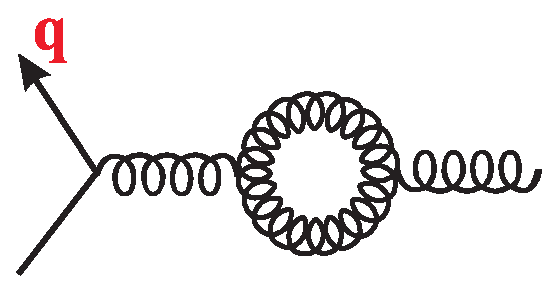
\includegraphics[scale=.33]{Afbeeldingen/GluonLoop.eps}
    \caption{Extra diagram bij QCD, dat voor \textit{antiscreening} zorgt. \cite{Martin}}
   \label{fig:GluonLoop}
  \end{center}
\end{figure}
QCD heeft nog een extra diagram dat de situatie iets moeilijker maakt, namelijk een vertex van drie gluonen, en bijhorende loop van pure gluonen (zie figuur \ref{fig:GluonLoop}).
Een fermion loop brengt afscherming van de (kleur)lading met zich mee (zie \ref{sec:QED}).
Een gluon loop zorgt voor \textit{antiscreening}, waardoor  $\alpha_S$ stijgt naarmate $Q^2$ kleiner wordt.
Dit volgt uit de uitdrukking voor $\alpha_S$, analoog aan \eqref{eq:alpha}:
\begin{align}
\alpha_S( Q^2 ) =\frac{\alpha(\mu^2)}{1+b_0 \alpha(\mu^2) \ln{\frac{Q^2}{\mu^2}}}
\end{align}
Hier heeft de coëfficiënt dus het tegengestelde teken, waar de tegenstelling tussen QED en QCD uit volgt.
Dit kan men herschrijven zodat de enige vrije parameter van QCD naar voor komt (zie bijvoorbeeld \cite[sectie 6.6]{Bettini}):
\begin{align} \label{eq:runningAlphaS}
\alpha_S(Q^2) = \frac{12\pi}{(33-2n_f) \ln{\frac{|Q|^2}{\lambda_\text{QCD}}}}
\end{align}
Waarbij $\lambda_\text{QCD}$ de fundamentele parameter in QCD is, die uit experimentele metingen wordt bepaald.
$\lambda_\text{QCD}$ hangt af van het aantal soorten quarks die bijdragen aan het proces $n_f$ (\cite[sectie 6.6]{Bettini}):
\begin{align}
\lambda_\text{QCD} = \mu^2 exp \left[ \frac{-12\pi}{(33-n_f) \alpha_S(\mu^2)} \right]
\end{align}
Voor drie en vier quarksoorten is $\lambda_\text{QCD}$ respectievelijk ongeveer gelijk aan 400 en 200 MeV.
Waarbij $\mu^2$ een schaalvariabele is waarvoor de koppeling gekend is.
$\lambda_\text{QCD}$ is zeer invloedrijk in verdere QCD berekeningen.
Als de energie kleiner is dan $\lambda_\text{QCD}$, is $\alpha_S$ groot en kan men geen perturbatieve berekeningen uitvoeren.
Daarbij komt dat $\alpha$ en $\alpha_S$ niet rechtstreeks gemeten kunnen worden, maar enkel door een theoretische berekening uit experimentele data kunnen worden afgeleid.
$\alpha_S$ zal dan bijgevolg minder nauwkeurig zijn, wegens zijn relatieve grootte.

    \subsubsection{Renormalisatiegroep vergelijking}
Omdat de keuze van $\mu^2$ in een berekening onmogelijk de gemeten waarde van een observabele kan beïnvloeden, moet er expliciet voor gezorgd worden door middel van de \textit{renormalisation group equation}:
\begin{align} \label{eq:RGE}
\frac{d R}{d\ln{\mu^2}} = \left(\frac{\partial}{\partial \ln{\mu^2}} + \frac{\partial \alpha_S}{\partial \ln{\mu^2}} \frac{\partial}{\partial \alpha_S} \right) R \notag \\
\Rightarrow R(Q^2/\mu^2, \alpha_S(Q^2)) = R(1,\alpha_S(Q^2))
\end{align}
Dit laatste betekent dat de twee afhankelijkheden (op $Q^2/\mu^2$ en $\alpha_S(\mu^2)$) eigenlijk maar een enkele zijn, namelijk het verloop van $\alpha_S(Q^2)$. Voor een uitwerking van de dubbele pijl in \eqref{eq:RGE} zie appendix \ref{app:RGE}).

    \subsubsection{QCD observabelen}
      \paragraph{}
Elke observabele kan in perturbatieve QCD ontwikkeld worden in machten van $\alpha_S$.
Bijkomende factoren zullen gevormd worden door logaritmes van $Q^2$ en bij lage $x$, $1/x^2$.
Omdat een observabele per definitie een eindig getal moet zijn, moeten de op eerste zicht divergente reeksen in $\alpha_S$ gehersommeerd worden.
Deze hersommatie kan enkel in speciale gevallen gebruikt worden, en alle tot nu toe bekende vormen zijn enkel in een bepaald regime (van $Q^2$ en/of $x$) geldig.
Omdat de exacte techniek op z’n minst moeilijk en zeer technisch is, worden hieronder enkel een beschrijving van de benaderingen en hun resultaten besproken. (\cite[sectie 9.5.2]{Barone})

      \paragraph{LLA}
\textit{Leading $\ln{Q^2}$ approximation}, waar de termen van de vorm $\alpha_S^n \ln^n{Q^2}$ gehersommeerd worden:
\begin{align} \label{eq:LLA}
R = \sum_n \alpha_S \ln^n{Q^2} \left( \sum_{k=n}^0 \ln^k{\frac{1}{x}} \right)
\end{align}
Dit leidt tot de DGLAP evolutievergelijkingen, die de evolutie van een observabele beschrijft in $Q^2$ bij “normale” $x$.
Indien ook termen van de vorm $\alpha_S^n \ln^{n-1}{Q^2}$ behouden blijven, krijgt men \textit{next-to leading $\ln{Q^2}$ approximation} en bijgevolg de NLLA DGLAP vergelijkingen.

      \paragraph{DLLA}
\textit{Double leading log approximation} duidt op het feit dat termen van de vorm $\alpha_S \ln^n{Q^2} \ln^n{\frac{1}{x}}$ behouden blijven:
\begin{align}
R = \sum_n \alpha_S \ln^n{Q^2} \ln^n{\frac{1}{x}}
\end{align}

      \paragraph{LL$_x$A}
In de praktijk zal voor heel lage $x$, $Q^2$ klein zijn, en men enkel de termen van de vorm $\alpha_S^n \ln^n{\frac{1}{x}}$ behoudt. Zo krijgt men de \textit{leading $\ln{\frac{1}{x}}$ approximation}:
\begin{align}
R = \sum_n \alpha_S \ln^n{\frac{1}{x}} \left( \sum_{k=n}^0 \ln^k{Q^2} \right)
\end{align}
\eqref{eq:LLA} en bovenstaande vergelijking zijn symmetrisch ten opzichte van $Q^2$ en $1/x$. Deze laatste leidt ook tot een veel bestudeerde BFKL evolutievergelijking.

      \paragraph{Parton dichtheden}
Een probleem in de recente resultaten van DGLAP berekeningen tot \textit{next-to next-to leading order}, is het opblazen van de parton dichtheden in een proton voor zeer kleine $x$.
In figuur \ref{fig:PD} staat voor twee verschillende schalen $Q^2$ getoond wat de dichtheden van de verschillende partons (gluonen en (zee)quarks) in het proton zijn.
Als dit verloop blijft doorgaan, zullen dichtheden optreden die niet meer fysisch zijn (unitariteit is niet meer geldig), waardoor de kans om met een parton te botsen groter dan 1 kan zijn.
\begin{figure} [H]
  \begin{center}
    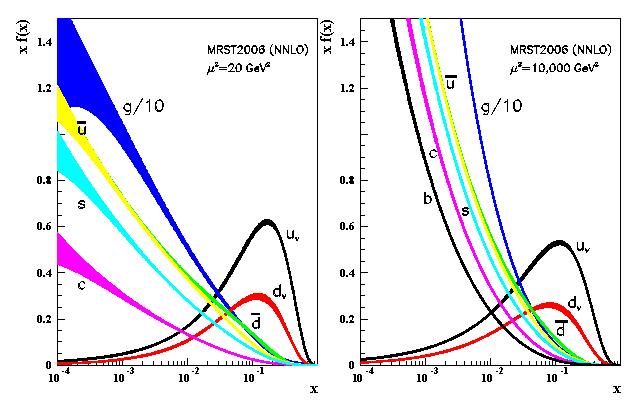
\includegraphics[scale=1]{Afbeeldingen/PD.eps}
    \caption{Dichtheden van de verschillende partonen in een proton voor twee verschillende schalen $Q^2$. Voor kleine $x$ gaan de gluonen sterk domineren. Voor relatief grote $x$-waarden vindt men de klassieke $uud$ combinatie terug, met de gluonen en zeequarks sterk onderdrukt. \cite{Martin}}
   \label{fig:PD}
  \end{center}
\end{figure}

    \subsubsection{DGLAP en BFKL}
Evolutievergelijkingen geven het verband tussen een grootheid (bijvoorbeeld een dichtheidsfunctie van quarks of gluonen) bij een (bijna) willekeurige waarde van $Q^2$ of $x$ en de waarde van de grootheid bij een bekende $Q_0^2$ of $x_0^2$.

      \paragraph{DGLAP}
De DGLAP vergelijkingen kunnen gebruikt worden om de quark- en gluondichtheden voor een hogere waarde van $Q^2$ te berekenen, indien deze dichtheden bij een kleinere waarde $Q_0^2$ bekend zijn.
De $x$-afhankelijkheid is hier onbekend, en moet experimenteel worden vastgesteld.

      \paragraph{BFKL}
De BFKL vergelijkingen doen net het omgekeerde: als de dichtheden bij een bepaalde waarde $x_0$ bekend is (hier moeten bepaalde aannames gemaakt worden, omdat bij lage $x$ niets exact berekend kan worden), kunnen e dichtheden berekend worden voor (bijna) willekeurige $x$.
Net zoals bij DGLAP de $x$-afhankelijkheid niet bekend was, blijft bij BFKL de $Q^2$-afhankelijkheid onbekend.

      \paragraph{Geldigheid}
Zoals al aan te voelen was, is elke vorm van evolutie maar geldig in een bepaald geval (kleine $x$, grote $Q^2$), net door de aanname die gemaakt werd bij het hersommeren van de reeks in $\alpha_S$.
In figuur \ref{fig:DGLAP-BFKL} wordt aangeduid wanneer welke vergelijkingen aangewezen zijn.
\begin{figure} [H]
  \begin{center}
    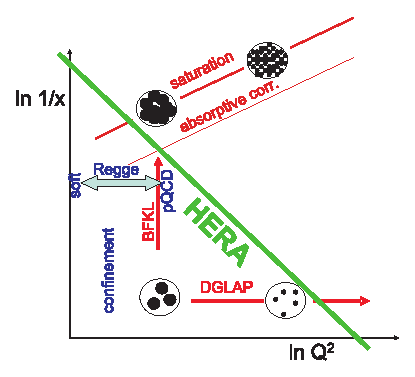
\includegraphics[scale=1]{Afbeeldingen/DGLAP-BFKL.eps}
    \caption{Schematische weergave van wat met verschillende benaderingen kan verwezenlijkt worden. Regge duidt op een gebied waar een pre-QCD theorie (Regge-theorie) geldig is. pQCD slaagt op perturbatieve QCD. \cite{Martin}}
   \label{fig:DGLAP-BFKL}
  \end{center}
\end{figure}
In figuur \ref{fig:DGLAP-BFKL} kan men ook een saturatielijn zien, die een theoretisch voorspelde grens vormt, waar saturatie van de partondistributies belangrijk zou worden (zie figuur \ref{fig:PD}).
De quark- en gluondistributies geven aanleiding tot structuurfuncties, die de structuur van een groter object (hier een proton) kunnen beschrijven bij bepaalde $Q^2$ en $x$.

    \subsection{Structuurfuncties}
Een meetbare grootheid die de theorie verbindt met harde waarnemingen, is de structuurfunctie.
Deze waarschijnlijkheidsverdelingen in functie van $x$ en $Q^2$  geven een indicatie van de kans om in een DIS proces met een parton te botsen met die $x$ en $Q^2$.
Met de juiste definities kan men de werkzame doorsnede voor een NC proces (figuur \ref{fig:NC}) als volgt schrijven (als $M^2/Q^2 \rightarrow 0$):
\begin{align} \label{eq:SF}
\frac{d\sigma}{dxdQ^2} &= \frac{2\pi \alpha^2}{xQ^4} \left(Y_+ F_2 \pm Y_- x F_3 - y^2 F_L \right)
\end{align}
Een uitgebreide discussie van bovenstaande uitdrukking staat in appendix \ref{app:SF}.
Als er enkel een foton kan worden uitgewisseld ($\sigma_\gamma \gg \sigma_Z$, dus de interactie via Z wordt verwaarloosd), kan men aantonen dat $F_3 \approx 0$ (zie ook appendix \ref{app:SF}).
In dit werk zal gekeken worden naar het gebied met heel kleine $x$, waardoor saturatie belangrijk wordt.

    \subsubsection{Saturatie} \label{sec:Saturatie}
Saturatie zal in een of andere vorm moeten optreden voor zeer kleine $x$, omdat anders de partondichtheden niet fysisch meer zijn en de huidige formulering onzinnige resultaten zou voorspellen (zie figuur \ref{fig:PD}).
In dit werk wordt dus uitbundig gebruik gemaakt van modellen die met dit fenomeen rekening houden.
Een beproefd en op zich eenvoudig model, is dat van Krzysztof Golec-Biernat \cite{GB}.
Golec-Biernat gebruikt het formalisme van de foton golffunctie, waarbij een foton onafhankelijk van de DIS botsing kan splitsen in een $q\bar{q}$-paar, dat dan interageert met het proton.
Dit laat toe een perturbatieve berekening te doen voor deze golffunctie, en de rest wordt beschreven door middel van een model.
\begin{align}
\sigma_{T,L} = \int d^2 \vec{r} \int_0^1 dz |\Psi_{T,L} (z, \vec{r})|^2 \hat{\sigma} (x,r^2)
\end{align}
Waarbij $\Psi$ de golffunctie van het foton is, $T$ en $L$ duiden op respectievelijk het longitudinaal en het transversaal deel hiervan, en $\hat{\sigma}$ het gemodelleerde, niet-perturbatieve gedeelte is.
Bovenstaande vergelijking is geformuleerd in positieruimte.
$r$ is de afstand tussen het ontstane $q\bar{q}$-paar.
Golec-Biernat en Wüsthoff bespreken in \cite{GBW} wat het GBW model wordt genoemd.
Dit model kan in impulsruimte en in positieruimte gebruikt worden.
De saturatie zit in de factor $\hat{\sigma}$, die de volgende vorm heeft:
\begin{align}
\hat{\sigma}(x,r^2) &= \sigma_0 \left[ 1- \exp{\left(-\frac{r^2}{4 R_0^2(x)}\right)} \right] \\
R_0^2(x) &= \frac{1}{Q_0^2} \left( \frac{x}{x_0} \right)^\lambda \label{eq:R0}
\end{align}
\eqref{eq:R0} is de \textit{saturation radius}, wat effectief een saturatie schaal invoert voor $r$.
$Q_0^2$ is 1 GeV, en ingevoerd om de juiste dimensies te krijgen.
$\sigma_0$, $\lambda$ en $x_0$ zijn de parameters van het model, die bepaald zijn door te fitten aan alle DIS data die beschikbaar was.
Ze verschillen voor het geval waar enkel $uds$ quarks bijdragen en waar ook de charm quark bijdraagt (zie appendix \ref{app:GBWparameters}).
Dit model heeft een ingebouwde begrenzing van de dipool werkzame doorsnede $\hat{\sigma}$.
Deze heeft het juiste gedrag in $r$: kwadratisch voor kleine $r$, en constant voor grote waarden.
Dat $\hat{\sigma}$ nul is voor kleine dipoolstraal $r$, hoeft geen verwondering.
Als de afstand $r$ tussen de twee quarks van $q\bar{q}$-paar klein is, zal het vanop redelijke afstand een kleurneutraal object vormen en kan er dus geen QCD interactie optreden.
Dit effect heet kleurdoorzichtigheid.
Een ander sterk punt van dit model is het feit dat hier een saturatie voor kleine $x$ is ingebouwd, wat natuurlijk wenselijk is voor berekeningen in dat gebied.

  \subsection{Dwarse energiestroom}
    \subsubsection{Belang voor LHeC}
    \subsubsection{Formulering}
In \cite{ET} wordt een uitdrukking berekend voor de transversale energiestroom van een DIS botsing.
Deze uitdrukking werd berekend voor kleine $x$ (dus met behulp van BFKL dynamica), en ingevuld met vergelijkingen die toen de beste resultaten gaven.
Hier zal deze vergelijking herbekeken worden, en toegepast op hernieuwde uitdrukkingen voor de bestanddelen.
\begin{align} \label{eq:ET}
x_j \frac{\partial E_T}{\partial x_j} = \frac{1}{F_2} \int \frac{dk_p^2}{k_p^2} \int \frac{dk_\gamma^2}{k_\gamma^2} \left( \frac{3\alpha_S}{\pi} \right) \mathcal{F}_2 \left( \frac{x}{x_j}, k_\gamma^2, Q^2 \right) f(x_j,k_p^2) \int \frac{d\phi}{\sqrt{k_p^2+k_\gamma^2+2k_p k_\gamma \cos{\phi}}}
\end{align}
Deze uitdrukking bestaat uit verschillende, af te zonderen delen, waar later meer aandacht zal worden aan besteed.
$F_2 (x, Q^2)$ is de structuurfunctie van het proton, $f$ is de dichtheid van het gluon en $\mathcal{F}_2$ is de structuurfunctie van de hadronische structuur van het foton.
Belangrijk op te merken is dat $F_2$ op voorhand kan berekend worden, en de integraal over $\phi$ analytisch kan worden bepaald.
Dit laat op eerste zicht nog maar 2 integraties over om numeriek te berekenen.


    
    \subsubsection{Gluon dichtheid}
    \subsubsection{$F_2$}
    \subsubsection{$\mathcal{F}_2$}


\section{Resultaten}

\section{Bespreking}

\section{Besluit}

\newpage
\appendix
\section{Diep Inelastische Verstrooiing} \label{app:DIS}
Als men figuur \ref{fig:DIS} beschouwt in het IMF ($m_e \approx m_p \approx 0$), geldt wegens behoud van energie:
\begin{align}
&(xP+q)^2 = m_e = 0 \notag \\
\Leftrightarrow &x^2 P^2 + 2xPq + q^2 = 0 \notag \\
\Leftrightarrow &2xPq -Q^2=0
\end{align}
Waarbij gebruikt is dat $-q^2 = Q^2 \gg x^2P^2$ in het  IMF. Dit laatste is equivalent met \eqref{eq:Bjorkenx}.

\section{DIS werkzame doorsnede} \label{app:SF}
Uit kwantum veldentheorie kan men de werkzame doorsnede voor een NC proces zoals in figuur \ref{fig:NC} halen:
\begin{align}
\frac{d\sigma}{dxdQ^2} &= xs \frac{d\sigma}{dxdQ^2} = \frac{2\pi y \alpha^2}{Q^4} \sum_j \eta_j L_j^{\mu \nu} W_{\mu \nu}^j
\end{align}
Waarbij de som over j loopt over
\begin{itemize}
  \item $\gamma$, met $\eta_\gamma=1$,
  \item $\gamma Z$, met $\eta_{\gamma Z} = \left( \frac{G_F M_Z^2}{2\sqrt{2}\pi \alpha} \right) \left(\frac{Q^2}{Q^2+M_Z^2} \right)$,
  \item $Z$, met $\eta_Z = \eta_{\gamma Z}^2$.
\end{itemize}
Hier stelt de tweede term de foton en Z uitwisseling voor, en de interferentie tussen de twee. $G_F$ is de Fermi koppeling en $\alpha$ de QED koppeling.
Er is naast $x$ en $Q^2$ nog een derde variabele nodig, die te maken heeft met de totale energie van het systeem.
Dit kan de Mandelstam variabele s zijn, of het relatieve energieverlies van het elektron in het massamiddelpuntsysteem y, zoals hieronder gedefinieerd.
\begin{align}
y &= \frac{p \cdot q}{p \cdot k} = \frac{\Delta E}{E} ,& s = (k+p)^2 \simeq \frac{Q^2}{xy}
\end{align}
$y$ wordt wel eens als \textit{rapidity} gebruikt, wat een Lorentz invariante parameter is voor de verstrooiingshoek $\hat{\theta}$ in het massamiddelpuntstelsel.
In dit geval geldt volgende relatie:
\begin{align}
y = \frac{1}{2} \left( 1-\cos{\hat{\theta}} \right)
\end{align}
$L^{\mu \nu}$ is de gekende tensor van het lepton knooppunt in functie van $k$ en $k'$.
$W_{\mu \nu}$ is een onbekende tensor van het hadron knooppunt.
Deze laatste kan dus enkel geparametriseerd worden aan de hand van wat wel gekend is.
De algemene uitdrukking ingeval van niet gepolariseerde DIS is als volgt:
\begin{align}
W_{\mu \nu} = \left( -g_{\mu \nu} + \frac{q_\mu q_\nu}{q^2} \right) F_1(x,Q^2) + \frac{\hat{P}_\mu \hat{P}_\nu}{p \cdot q} F_2(x,Q^2) -  i\epsilon_{\mu \nu \alpha \beta} \frac{q^\alpha p^\beta}{2p \cdot q} F_3(x,Q^2)
\end{align}
Hier zijn $F_i$ de structuurfuncties, afhankelijk van $x$ en $Q^2$.
De derde term bevat een uitwendig product (de $\vec{q} \times \vec{q}$ vorm), waardoor deze term pariteit niet behoudt.
Deze term zal dan ook $\approx 0$ indien de Z bijdrage verwaarloosbaar is, omdat voor zover gekend pariteit nog steeds behouden is voor de sterke wisselwerking.
Men bekomt \eqref{eq:SF} door $L^{\mu \nu}$ in te vullen en volgende variabelen te definiëren:
\begin{align}
Y_\pm &= 1 \pm (1-y)^2 \notag \\
F_L &= F_2 - 2x F_1 \notag
\end{align}
In DIS processen, kan men vaak uitgaan van $F_L = 0$, zodat $F_2$ voldoende is om de hele werkzame doorsnede te bepalen.

\section{Renormalisatiegroep vergelijking} \label{app:RGE}
Vergelijking \eqref{eq:RGE} wordt als volgt bekomen. Vertrekkende van het stuk voor de dubbele pijl, en volgende nieuwe variabele $t$ en functie $\beta$:
\begin{align}
t = \ln{\frac{Q^2}{\mu^2}}, \beta(\alpha_S) =  \frac{\partial \alpha_S}{\partial \ln{\mu^2}}
\end{align}

\section{Parameters van het GBW model voor saturatie} \label{app:GBWparameters}
In het geval van 3 lichte quarks: up, down en strange, krijgt men volgende waarden:
\begin{align}
\sigma_0 &= 23.03 \text{mb} \notag \\
\lambda &= 0.288 \\
x_0 &= 3.04 \times 10^{-4} \notag
\end{align}
In geval van een vierde charm quark zijn de gefitte waarden anders.
\begin{align}
\sigma_0 &= 29.12 \text{mb} \notag \\
\lambda &= 0.277 \\
x_0 &= 0.41 \times 10^{-4} \notag
\end{align}
De waarden komen overeen met die in \cite{GBW}.

\newpage
\begin{thebibliography}{99}

\bibitem{Martin}
  Alan D. Martin,
  \emph{Proton Structure, Partons, QCD, DGLAP, and Beyond}.
  Institute for Particle Physics Phenomenology,
  University of Durham
  Durham, DH1 3LE, UK
  12 mei, 2008.

\bibitem{Bettini}
  Alessandro Bettini
  \emph{Introduction to Elementary Particle Physics}
  Cambridge University Press
  2008

\bibitem{Barone}
  Vincenzo Barone, Enrico Predazzi
  \emph{High-energy particle diffraction}
  Springer-Verlag Berlin Heidelberg New York
  2002

\bibitem{GB}
  Krzysztof Golec-Biernat
  \emph{Deep Inelastic Scattering at Small Values of the Bjorken Variable x}
  Habilitation thesis,
  Kraków/Hamburg
  2001

\bibitem{GBW}
  K. Golec-Biernat, M. Wüsthoff
 \emph{ Saturation Effects in Deep Inelastic Scattering at low $Q^2$ and its Implications on Diffraction}
  2008
  
\bibitem{ET}
  J.Kwieciński, A.D. Martin, P.J. Sutton, K. Golec-Biernat
  \emph{QCD predictions for the transverse energy flow in deep-inelastic scattering in the DESY HERAsmall $x$ regime}
  Physical Review D, Volume 50, 1
  1994

\end{thebibliography}

\end{document}
